\section{Relative Error Analysis}
\label{sec:erroranalysis}

\subsection{Topic I}
\label{subsec:first_topic_error}

\begin{center}
   \begin{tabular}{|c|||c|c|c|}
      \hline    
      \multicolumn{4}{|c|} {\bf ANALISE DO ERRO COM 4 COLUNAS} \\
      \hline
        
 Node 1 & 5.029246e+00         & 5.02924600001e+00 & 1.98836979289e-10 \\ \hline 
 Node 2 & 4.783544e+00         & 4.78354415384e+00 & 3.21593851440e-06 \\ \hline 
 Node 3 & 4.288147e+00        & 4.28814736170e+00 & 8.43484611997e-06 \\ \hline 
 Node 4 & 4.817533e+00         & 4.81753272504e+00 & 5.70752959068e-06 \\ \hline 
 Node 5 & 5.579905e+00         & 5.57990489781e+00 & 1.83143454860e-06 \\ \hline 
 Node 6 & -1.85471e+00         & -1.85471262435e+00 & 1.41496768946e-04 \\ \hline 
 Node 7 & -2.77162e+00         & -2.77162277031e+00 & 9.99527366038e-05 \\ \hline 
   \end{tabular}
 \end{center}
 
 
 
\subsection{Topic II}
\label{subsec:second_topic_error}

\begin{center}
   \begin{tabular}{|c|||c|c|c|}
      \hline    
      \multicolumn{4}{|c|} {\bf ANALISE DO ERRO COM 4 COLUNAS PARA O 2} \\
      \hline
        Merit Figure & 0.000410 
   \end{tabular}
 \end{center}
 
 
\subsection{Topic III}
\label{subsec:third_topic_error}

\begin{figure}[H]

\begin{subfigure}{0.5\textwidth}
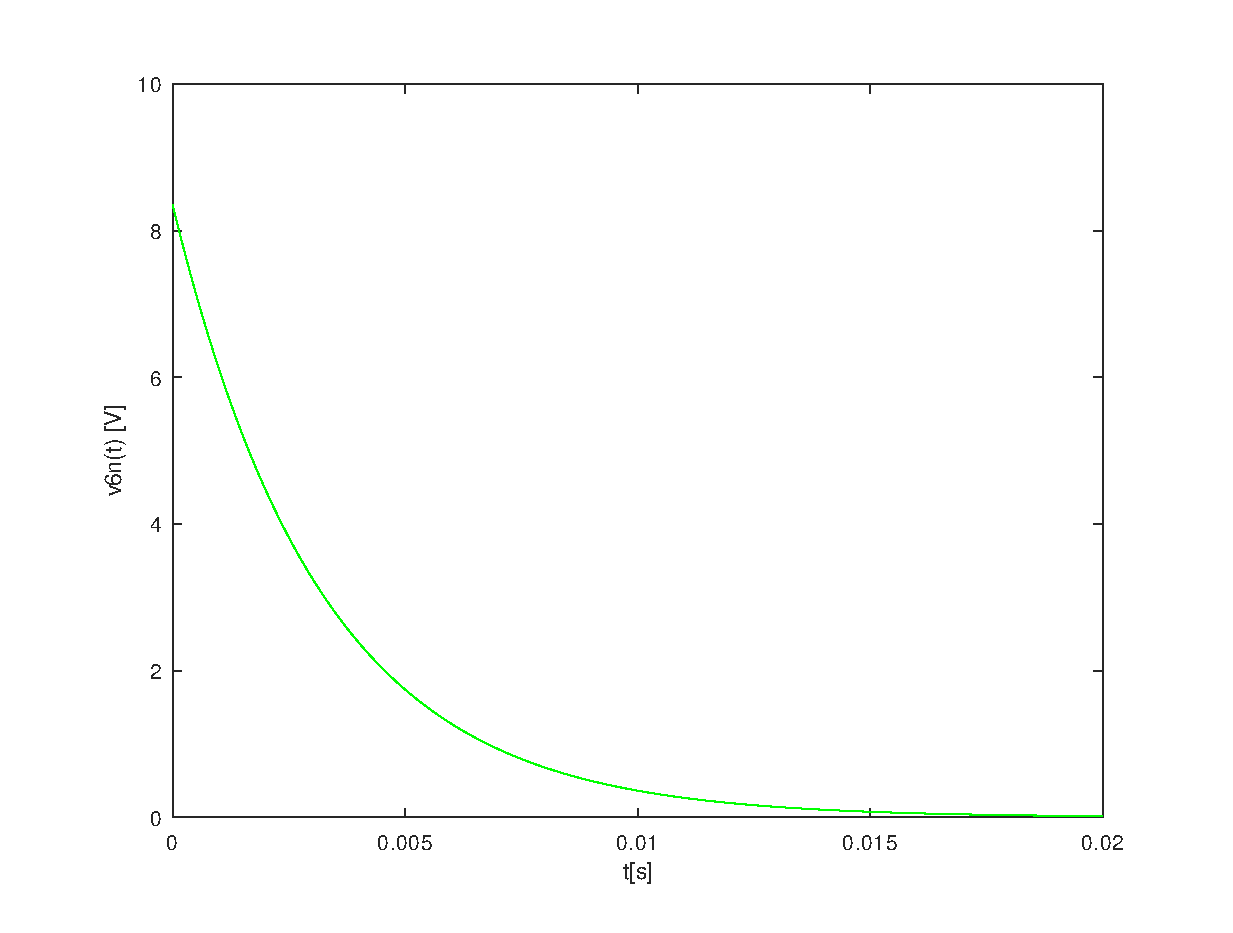
\includegraphics[width=0.9\linewidth, height=6cm]{natural.eps} 
\caption{The natural solution, $V6_n(t)$, during time interval [0, 20] ms, obtained using GNU Octave.}
\label{fig:theo_third}
\end{subfigure}
\begin{subfigure}{0.5\textwidth}
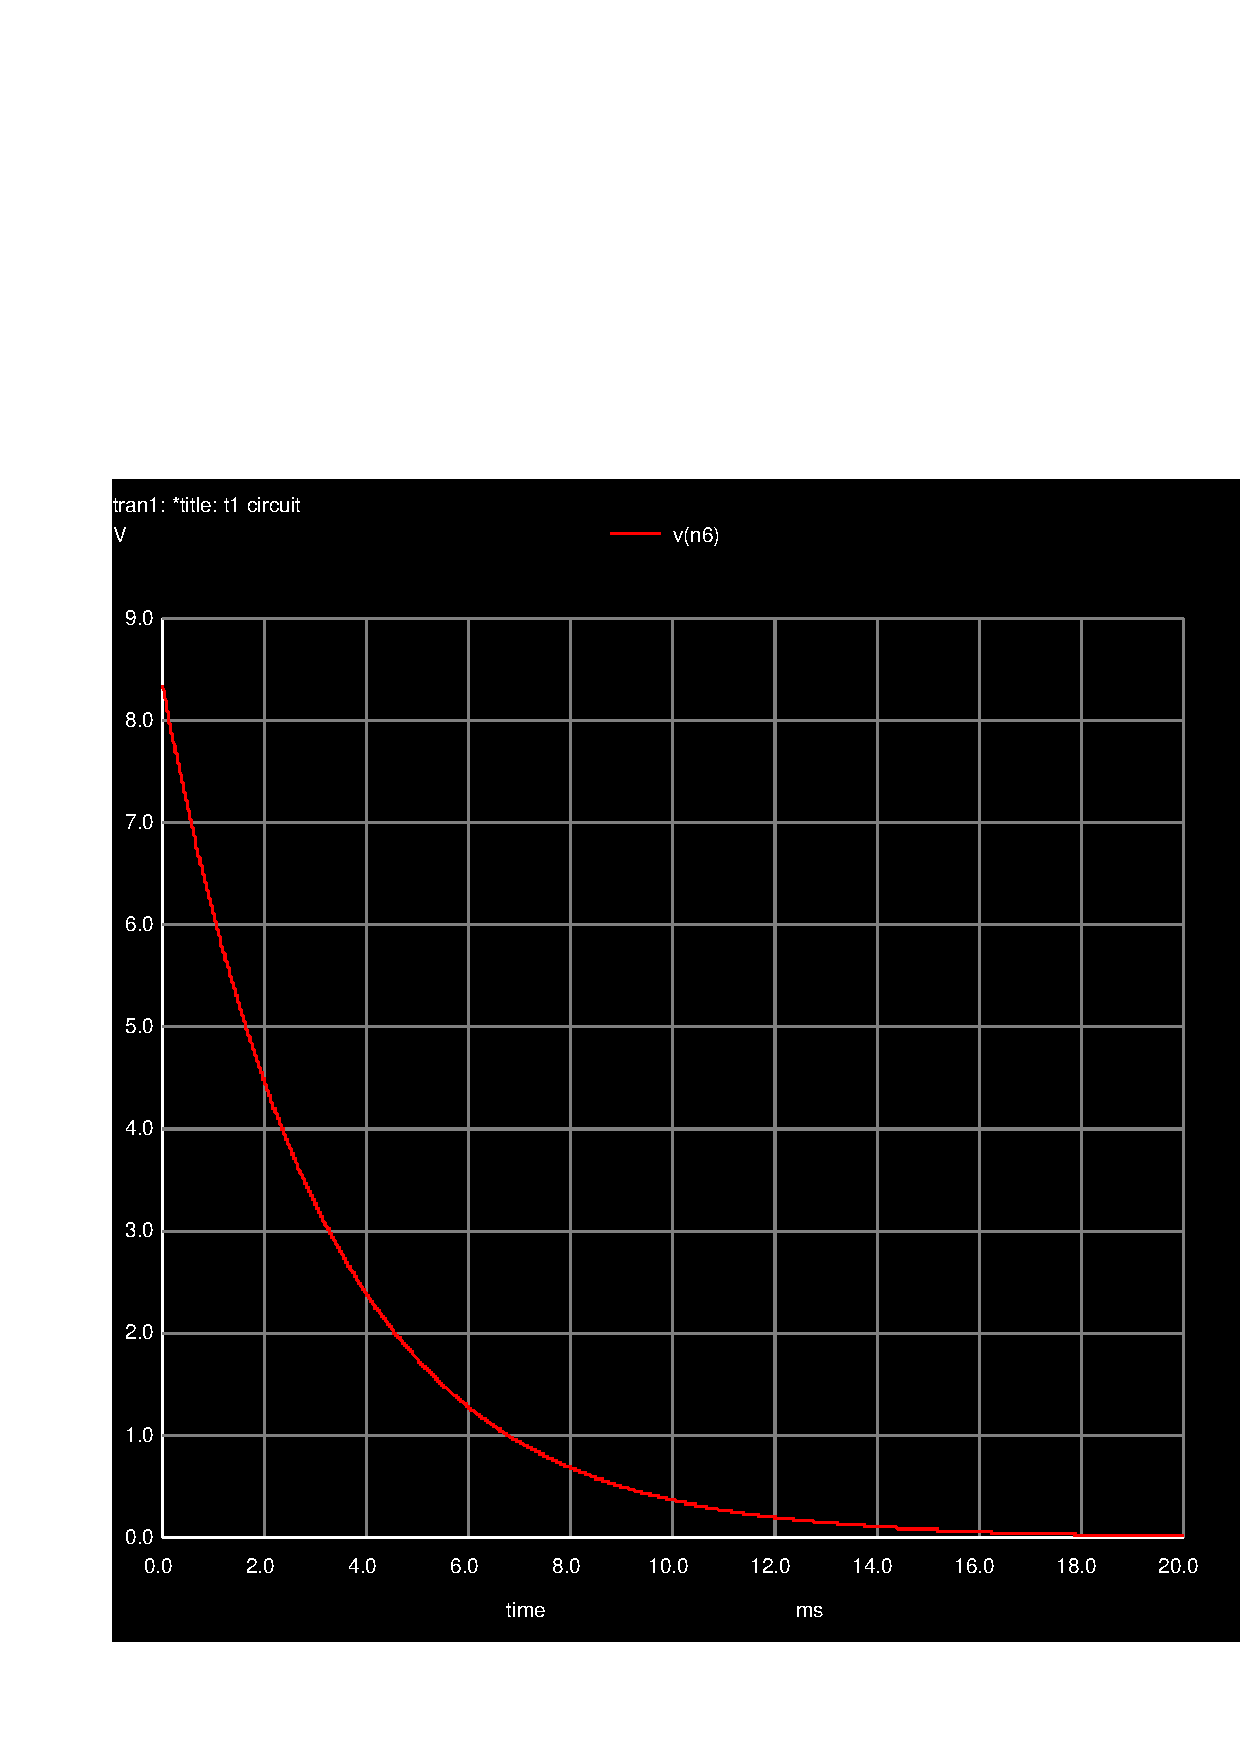
\includegraphics[width=0.9\linewidth, height=6cm]{trans1.pdf}
\caption{The natural solution, $V6_n(t)$, during time interval [0, 20] ms, obtained using Ngspice.}
\label{fig:natural}
\end{subfigure}

\caption{Comparation of theoretical and simulation analysis for the natural response.}
\label{fig:compar_1}
\end{figure}


\subsection{Topic IV}
\label{subsec:fourth_topic_error}

\begin{figure}[H]

\begin{subfigure}{0.5\textwidth}
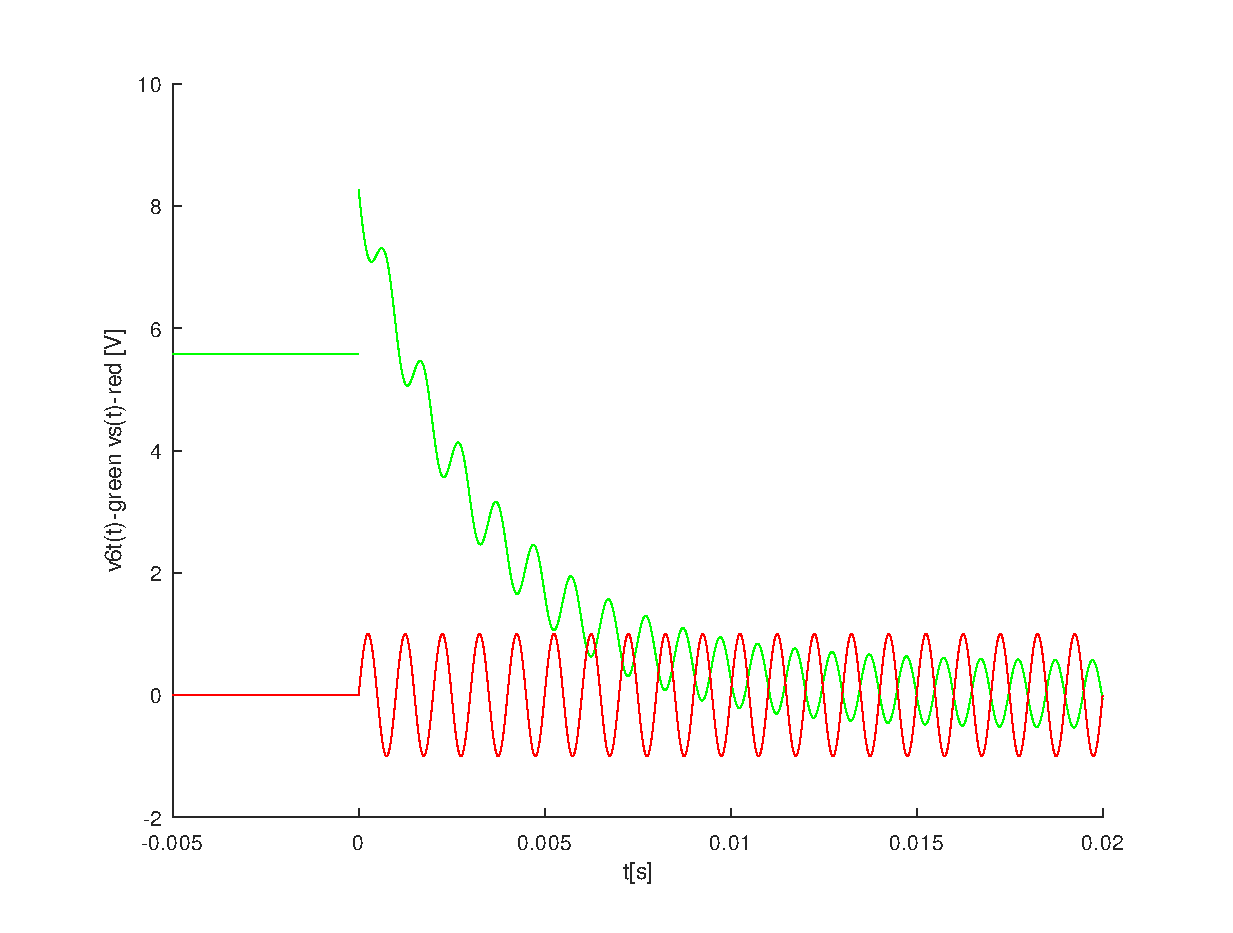
\includegraphics[width=0.9\linewidth, height=6cm]{total.eps} 
\caption{The final total solution, $V6(t)$,  and $v_s(t)$ during time interval [-5, 20] ms, obtained using GNU Octave.}
\label{fig:theo_fifth}
\end{subfigure}
\begin{subfigure}{0.5\textwidth}
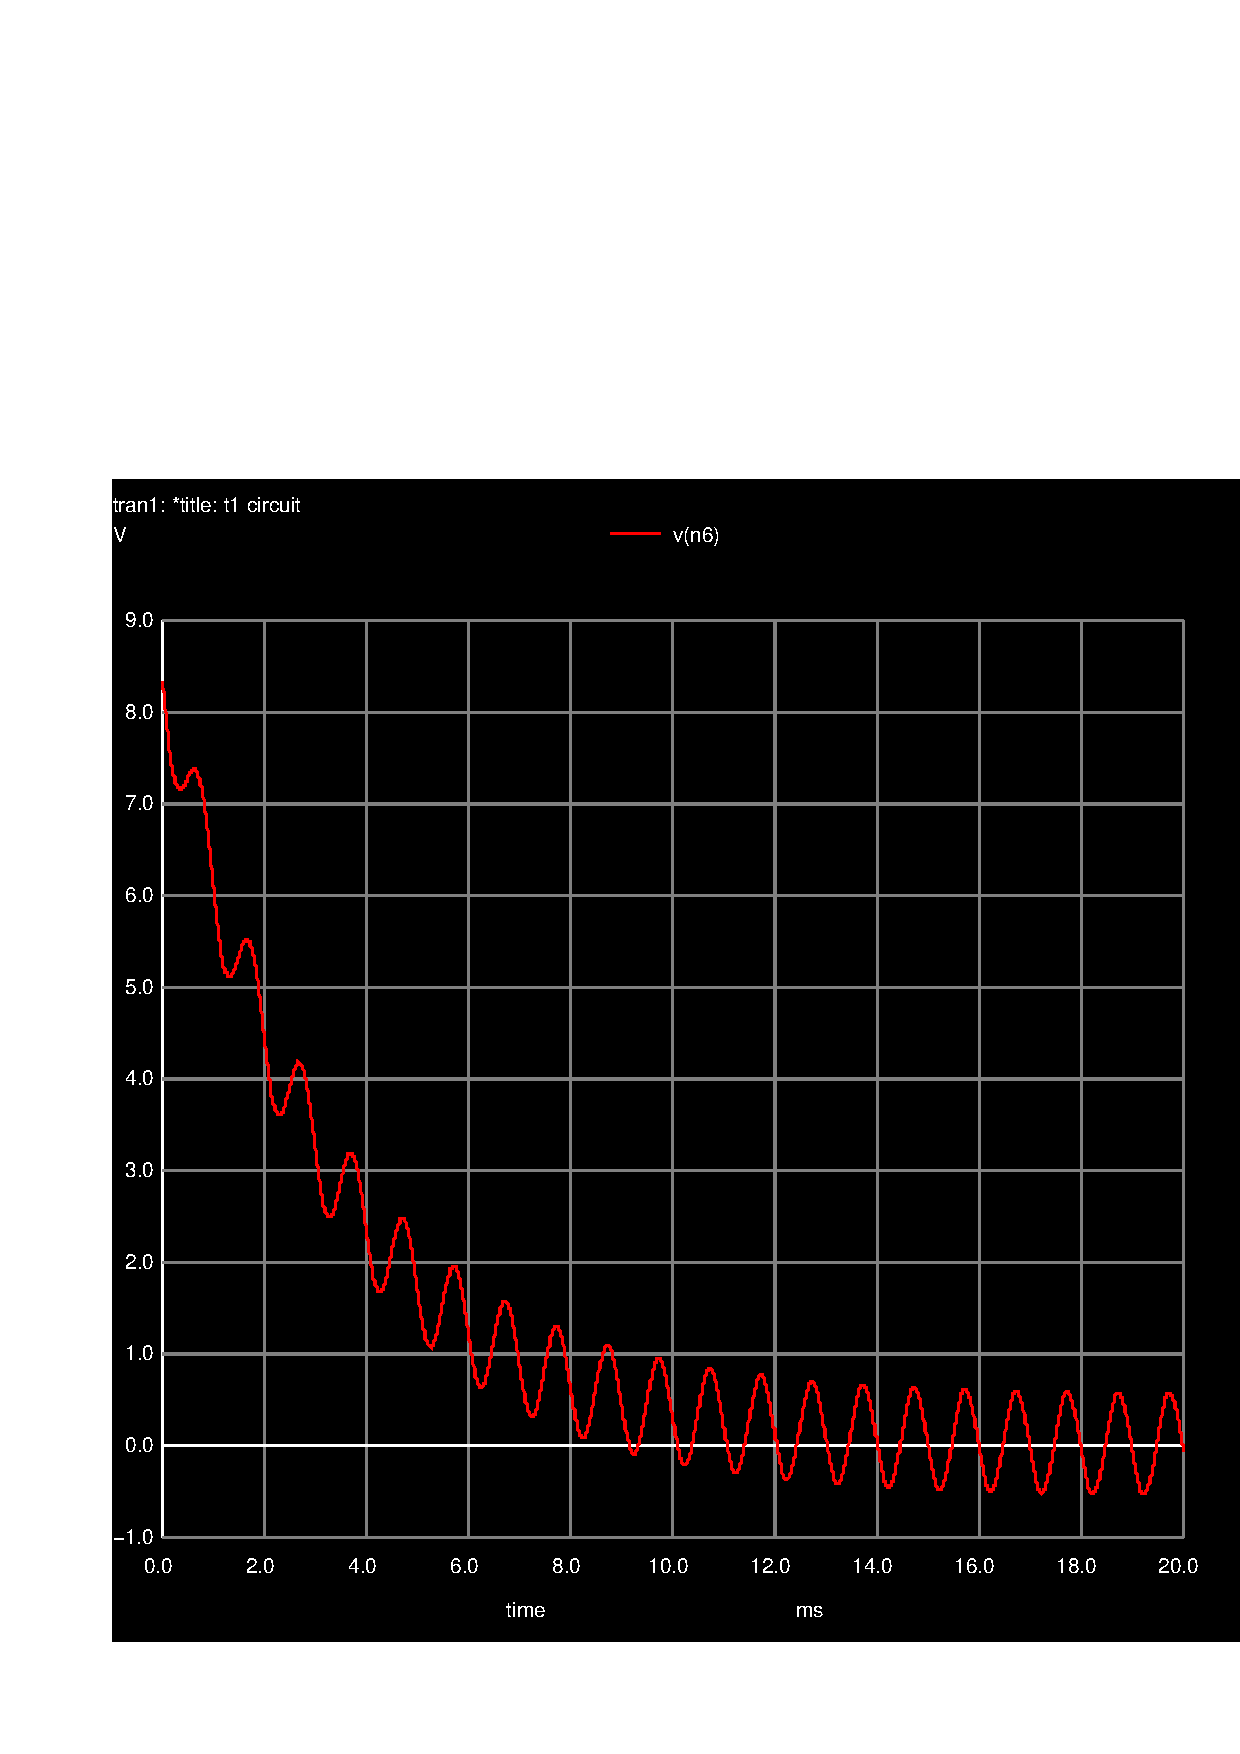
\includegraphics[width=0.9\linewidth, height=6cm]{trans2.pdf}
\caption{The final total solution, $V6(t)$,  and $v_s(t)$ during time interval [-5, 20] ms, obtained using Ngspice.}
\label{fig:total}
\end{subfigure}

\caption{Comparation of theoretical and simulation analysis for the total response.}
\label{fig:compar_2}
\end{figure}


\subsection{Topic V}
\label{subsec:fifth_topic_error}

\begin{figure}[H]

\begin{subfigure}{0.5\textwidth}
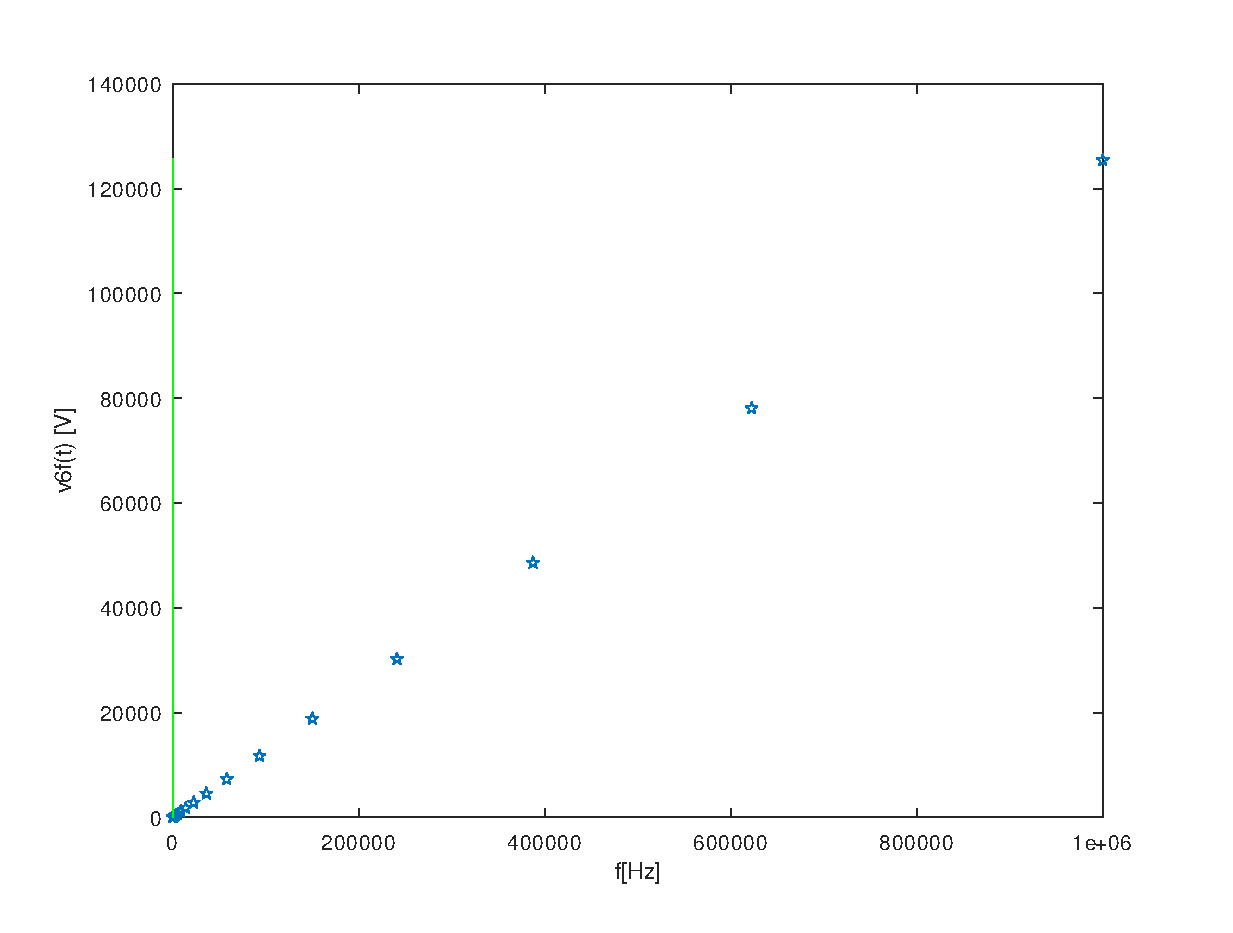
\includegraphics[width=0.9\linewidth, height=6cm]{magnitude.eps} 
\caption{Magnitude of $v_s(f)$,  $v_c(f)$  and $v_6(f)$ during frequency interval [0.1 , 1] MHz.}
\label{fig:theo_third}
\end{subfigure}
\begin{subfigure}{0.5\textwidth}
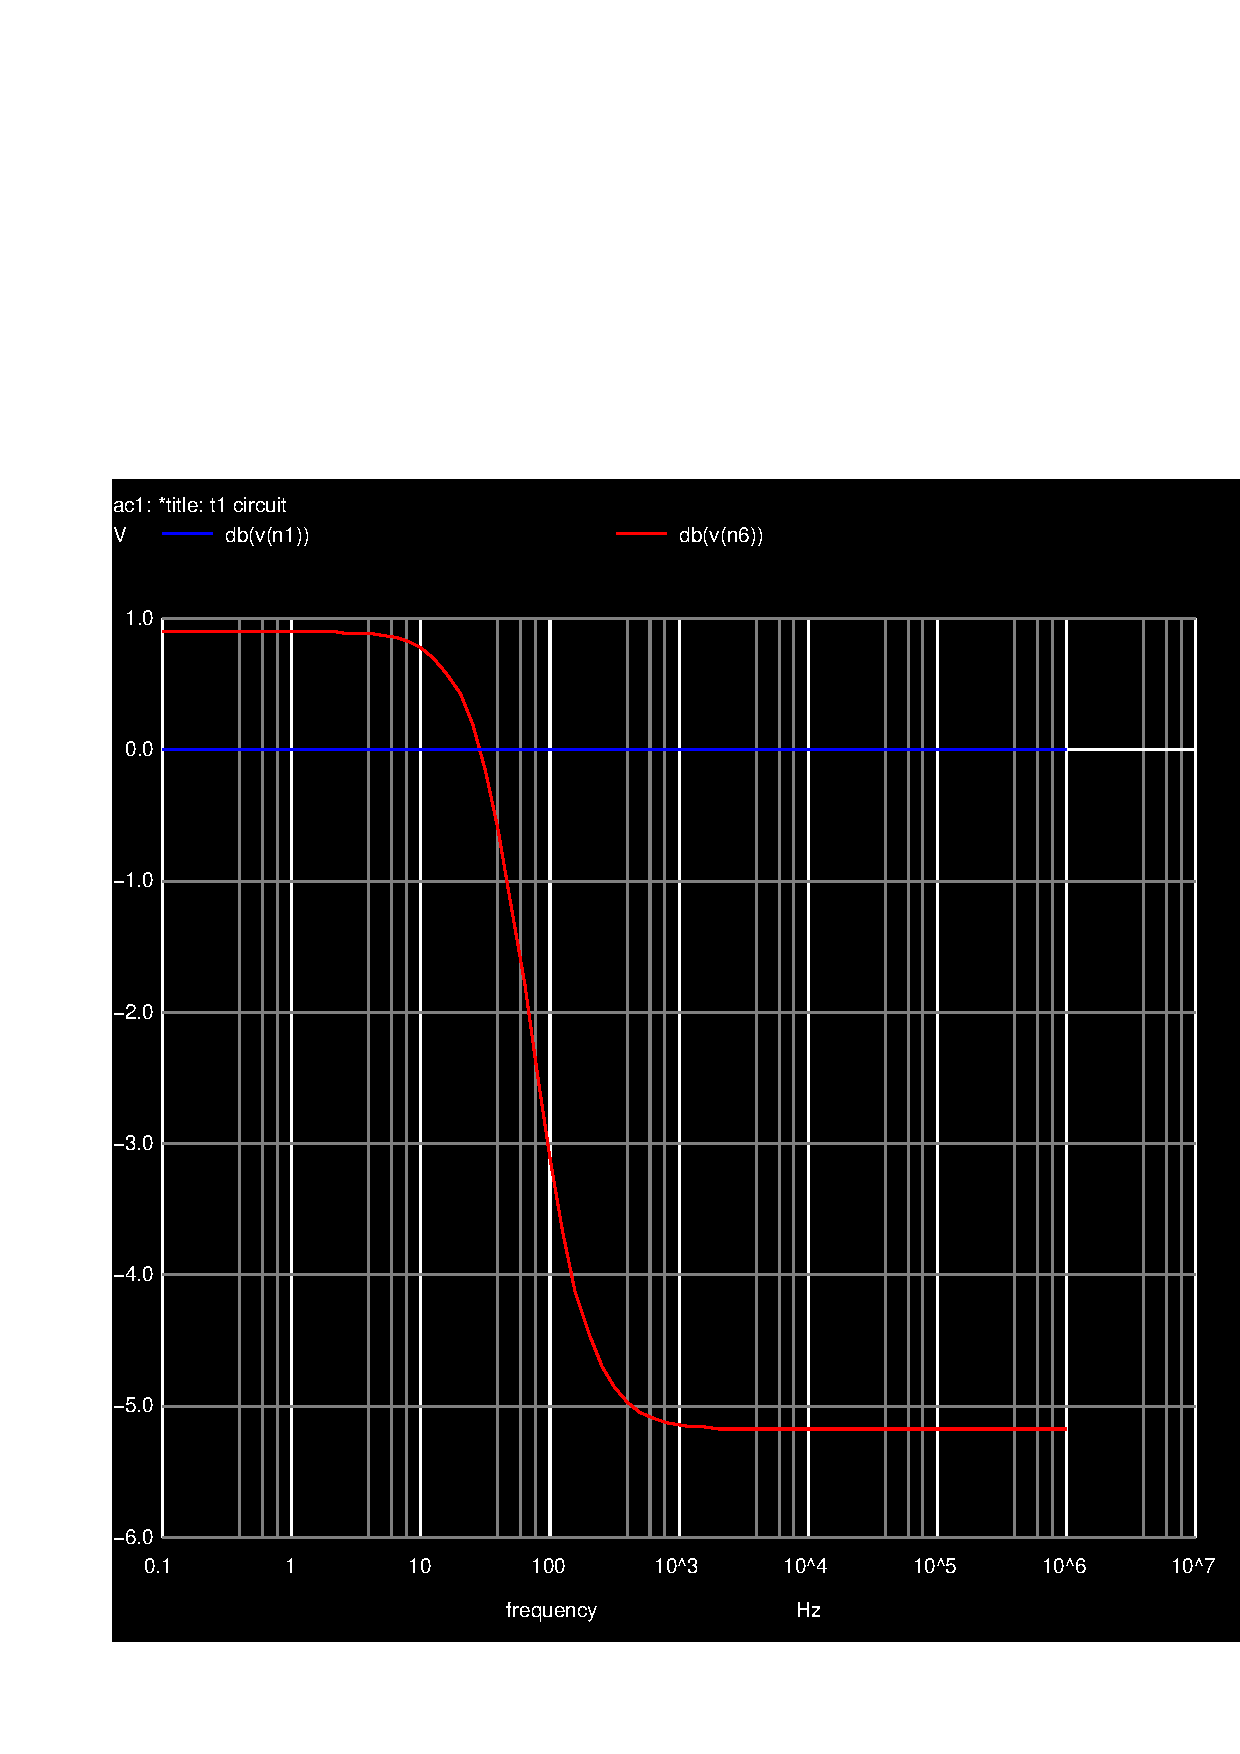
\includegraphics[width=0.9\linewidth, height=6cm]{acm.pdf}
\caption{The final total solution, $V6(t)$,  and $v_s(t)$ during time interval [-5, 20] ms, obtained using Ngspice.}
\label{fig:total}
\end{subfigure}

\caption{Comparation of theoretical and simulation analysis for the total response.}
\label{fig:compar_2}
\end{figure}




















